% This file was created with tikzplotlib v0.10.1.
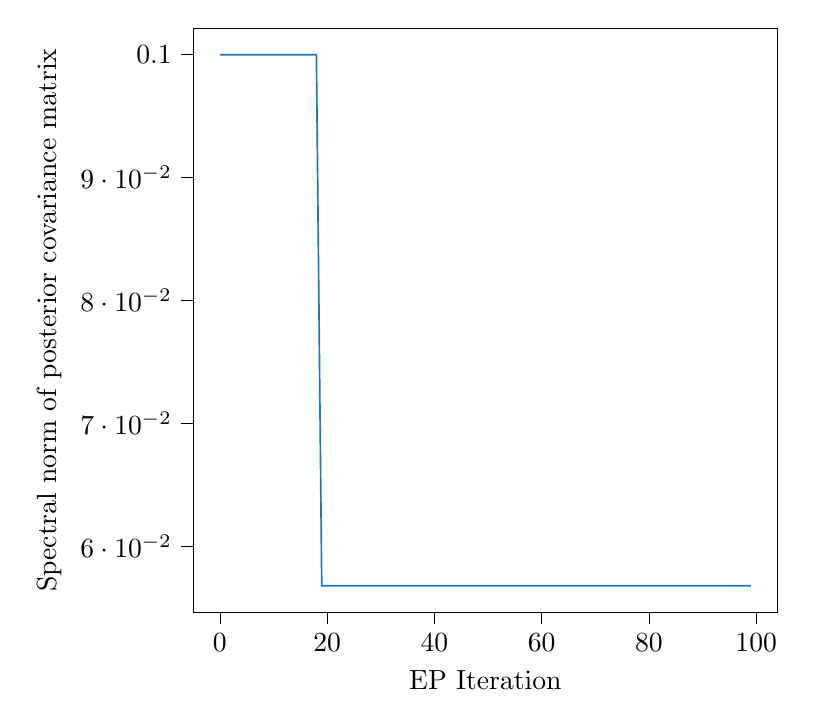
\begin{tikzpicture}

\definecolor{darkgray176}{RGB}{176,176,176}
\definecolor{steelblue31119180}{RGB}{31,119,180}

\begin{axis}[
height=9cm,
tick align=outside,
tick pos=left,
width=9cm,
x grid style={darkgray176},
xlabel={EP Iteration},
xmin=-4.95, xmax=103.95,
xtick style={color=black},
y grid style={darkgray176},
ylabel={Spectral norm of posterior covariance matrix},
ymin=0.0546158899864753, ymax=0.102161148095882,
ytick style={color=black}
]
\addplot [semithick, steelblue31119180]
table {%
0 0.1
1 0.1
2 0.1
3 0.1
4 0.1
5 0.1
6 0.1
7 0.1
8 0.1
9 0.1
10 0.1
11 0.1
12 0.1
13 0.1
14 0.1
15 0.1
16 0.1
17 0.1
18 0.1
19 0.0567770380823574
20 0.0567770380823574
21 0.0567770380823574
22 0.0567770380823574
23 0.0567770380823574
24 0.0567770380823574
25 0.0567770380823574
26 0.0567770380823574
27 0.0567770380823574
28 0.0567770380823574
29 0.0567770380823574
30 0.0567770380823574
31 0.0567770380823574
32 0.0567770380823574
33 0.0567770380823574
34 0.0567770380823574
35 0.0567770380823574
36 0.0567770380823574
37 0.0567770380823574
38 0.0567770380823574
39 0.0567770380823574
40 0.0567770380823574
41 0.0567770380823574
42 0.0567770380823574
43 0.0567770380823574
44 0.0567770380823574
45 0.0567770380823574
46 0.0567770380823574
47 0.0567770380823574
48 0.0567770380823574
49 0.0567770380823574
50 0.0567770380823574
51 0.0567770380823574
52 0.0567770380823574
53 0.0567770380823574
54 0.0567770380823574
55 0.0567770380823574
56 0.0567770380823574
57 0.0567770380823574
58 0.0567770380823574
59 0.0567770380823574
60 0.0567770380823574
61 0.0567770380823574
62 0.0567770380823574
63 0.0567770380823574
64 0.0567770380823574
65 0.0567770380823574
66 0.0567770380823574
67 0.0567770380823574
68 0.0567770380823574
69 0.0567770380823574
70 0.0567770380823574
71 0.0567770380823574
72 0.0567770380823574
73 0.0567770380823574
74 0.0567770380823574
75 0.0567770380823574
76 0.0567770380823574
77 0.0567770380823574
78 0.0567770380823574
79 0.0567770380823574
80 0.0567770380823574
81 0.0567770380823574
82 0.0567770380823574
83 0.0567770380823574
84 0.0567770380823574
85 0.0567770380823574
86 0.0567770380823574
87 0.0567770380823574
88 0.0567770380823574
89 0.0567770380823574
90 0.0567770380823574
91 0.0567770380823574
92 0.0567770380823574
93 0.0567770380823574
94 0.0567770380823574
95 0.0567770380823574
96 0.0567770380823574
97 0.0567770380823574
98 0.0567770380823574
99 0.0567770380823574
};
\end{axis}

\end{tikzpicture}
